\section{Experiments}


\subsection{Experimental Setup}


% main table comparing the baselines and our own methods

\begin{table*}[t]
\begin{center}
\begin{tabular}{ >{\raggedright\arraybackslash}p{3.9cm} c c c c c c c c } 
    \toprule

    \textbf{[Tuned] Model} & \textbf{Method }& \bm{$K$} & \textbf{Helpful} & \textbf{Clear} & \textbf{Factual} & \textbf{Deep} & \textbf{Engage} & \textbf{Avg.} \\
    \midrule

    [\xmark] Mistral 7b  & Base & 0 & 2.20 & 2.51 & 2.29 & 1.69 & 1.80 & 2.10 \\
    
   [\xmark] Mistral 7b  & URIAL & 3 & 3.62 & 4.32 & 3.75 & 2.70 & 3.41 &  3.56\\
    
    [\xmark] Mistral 7b  & \ours & 2 & \textbf{4.23} & \textbf{4.56} & \textbf{3.97} & \textbf{3.68} & \textbf{3.84} &  \textbf{4.06}\\
    
    \hline
    
   [\cmark] Mistral 7b (Instruct) & Base & 0 & 3.98 & 4.44 & 3.64 & 2.97 & 3.26 &  3.66\\
    
   [\cmark] Mistral 7b (Instruct) & URIAL & 3 & 3.94 & 4.51 & 3.69 & 2.99 & 3.75 &  3.78\\
    
    [\cmark] Mistral 7b (Instruct) & \ours & 2 & \textbf{4.22} & \textbf{4.60} & \textbf{3.80} & \textbf{3.68} & \textbf{3.99} &  \textbf{4.06}\\

   \hline

    [\xmark] Llama 2 70b$^q$  & Base & 0 & 2.07 & 2.55 & 2.35 & 1.50 & 1.63 &  2.02 \\
    
    [\xmark] Llama 2 70b$^q$ & URIAL & 3 & 4.25 & 4.67 & 4.03 & 3.08 & 3.80 &  3.97 \\
    
    [\xmark] Llama 2 70b$^q$  & \ours & 2 & \textbf{4.42} & \textbf{4.72} & \textbf{4.23} & \textbf{3.81} & \textbf{3.98} &  \textbf{4.23}\\

    \hline

    [\cmark] Llama 2 70b$^q$ (chat) & Base & 0 & 4.36 & 4.71 & 3.95 & 3.56 & 3.76 &  4.07\\

    [\cmark] Llama 2 70b$^q$ (chat) & URIAL & 3 & 4.32 & 4.72 & 4.08 & 3.50 & 4.25 &  4.17\\
    
    [\cmark] Llama 2 70b$^q$ (chat) & \ours & 2 & \textbf{4.46} & \textbf{4.75} & \textbf{4.10} & \textbf{4.11} & \textbf{4.37} &  \textbf{4.36}\\


   \hline

    [\xmark] Llama 3 8b  & Base & 0 & 1.82 & 2.27 & 2.20 & 1.38 & 1.48 &  1.83\\

    [\xmark] Llama 3 8b  & URIAL & 3 & 3.94 & \textbf{4.51} & 3.69 & 2.99 & \textbf{3.75} & 3.78 \\
    
    [\xmark] Llama 3 8b  & \ours & 2 & \textbf{4.02} & 4.40 & \textbf{3.84} & \textbf{3.50} & 3.65 &  \textbf{3.88} \\

   \hline

    [\cmark] Llama 3 8b (Instruct) & Base & 0 & 4.43 & 4.72 & 3.98 & 3.45 & 3.76 &  4.07\\

    [\cmark] Llama 3 8b (Instruct) & URIAL & 3 & 4.48 & 4.81 & \textbf{4.19} & 3.55 & 4.27 &  4.26\\
    
    [\cmark] Llama 3 8b (Instruct) & \ours & 2 & \textbf{4.54} & \textbf{4.81} & 4.16 & \textbf{4.08} & \textbf{4.40} & \textbf{4.40} \\

    \hline

    [\cmark] \texttt{gpt-3.5-turbo} & Base & 0 & 4.56 & 4.89 & 4.41 & 3.30 & 3.55 & 4.14 \\

    [\cmark] \texttt{gpt-3.5-turbo} & URIAL & 3 & 4.30 & 4.77 & 4.41 & 3.44 & 4.11 &  4.21\\
    
    [\cmark] \texttt{gpt-3.5-turbo} & \ours & 2 & \textbf{4.67} & \textbf{4.92} & \textbf{4.53} & \textbf{4.07} & \textbf{4.58} &  \textbf{4.55}\\

   \hline
    [\cmark] \texttt{gpt-4-0613} & Base & 0 & \textbf{4.71} & \textbf{4.93} & \textbf{4.52} & 3.49 & 3.53 &  \textbf{4.24} \\

    \bottomrule

\end{tabular}

\caption{Performance on \texttt{just-eval-instruct} benchmark. ``Tuned'' indicates whether the model has been SFT/RLHF tuned. Models are evaluated across multiple aspects: ``Helpful'' (Helpfulness), ``Clear'' (Clarity), ``Factual'' (Factuality), ``Deep'' (Depth), and ``Engage'' (Engagement). The base method indicates a basic alignment prompt. Our method consistently outperforms baseline methods across multiple aspects and overall.}
\label{tab:main_table}
\vspace{-17pt}
\end{center}
\end{table*}


\noindent \textbf{Evaluation Dataset}.
We use the standard alignment benchmark, \texttt{just-eval-instruct}~\cite{Lin2024ReAlign}, which merges five popular alignment datasets to provide a comprehensive and fine-grained evaluation of LLM alignment. This benchmark consists of 1,000 examples: the first 800 assess the models' helpfulness, and the remaining 200 evaluate their harmlessness. The first 800 examples are evaluated based on five fine-grained aspects: \textit{helpfulness}, \textit{clarity}, \textit{factuality}, \textit{depth}, and \textit{engagement}, while the remaining 200 are evaluated using the \textit{safety} aspect. We use GPT-4 Turbo (\texttt{gpt-4-1106-preview}), one of the latest GPT-4 models available during our experiments, to evaluate both types of examples using the prompts specified in the original URIAL paper~\cite{Lin2024ReAlign}. The scoring scale ranges from 1 to 5, indicating ``strongly disagree'', ``disagree'', ``neutral'', ``agree'', and ``strongly agree''. Note that we employ a more recent version of GPT-4 compared to URIAL, which enhances the strictness and accuracy of our evaluation pipeline. Thus, we re-benchmark URIAL under our updated evaluation setting for consistency across all results.


\noindent \textbf{Seed Samples}. 
When optimizing the system prompt with \ours, we sample from our seed dataset $\mathcal{X}$ to measure the alignment performance of the system prompt at each time step. This seed dataset, consisting of 180 examples, is built using data from \texttt{AlpacaEval} \cite{alpaca_eval}, \texttt{LIMA} \cite{zhou2024lima}, and \texttt{HH-RLHF-redteam} \cite{Ganguli2022RedTL}. More details about the construction of this dataset can be found in Appendix \ref{sec:impl_details}.


\noindent \textbf{Models}.
We benchmark 6 open-source LLMs in our experiments: Mistral 7b (v0.1), Mistral 7b (Instruct)~\cite{Jiang2023Mistral7}, Llama 2 70$b^q$, Llama 2 70$b^q$ (chat) (4-bit AWQ~\cite{lin2023awq} quantized models)~\cite{Touvron2023Llama2O}, Llama 3 8b, Llama 3 8b (Instruct)~\cite{llama3modelcard} and 2 closed-source models: OpenAI's GPT-3.5 Turbo (\texttt{gpt-3.5-turbo}) and GPT-4 (\texttt{gpt-4-0613}). Models without the ``chat'' or ``instruct'' tag are base models, i.e., not tuned by SFT/RLHF. For evaluation, we use greedy decoding (temperature = 0) to ensure reproducibility.



\noindent \textbf{Baselines}. 
We first apply \ours to the base model, making the SFT/RLHF-tuned counterparts without \ours a natural baseline. For instance, we compare Mistral 7B + \ours and Mistral 7b (Instruct). Additionally, we have two more baselines: (1) The base method, where a basic prompt is applied without using ICL examples. (2) URIAL~\cite{Lin2024ReAlign}, where we use the prompt and ICL examples proposed by authors. We also provide extensive ablation baselines of our method, such as changing the search algorithm from Beam search to Greedy Search or Monte Carlo search and using ``static rewarding'' to understand the impact of dynamic rewarding. Full details of these can be found in Appendix~\ref{sec:impl_details}.




\noindent \textbf{Implementation details}.
We use GPT-4-turbo (\texttt{gpt-4-0125-preview}) as both the optimizer $\mathcal{O}$, and evaluator $\mathcal{E}$ unless specified otherwise. The initial set of in-context learning examples, $\mathcal{I}_{base}$, contains 16 examples: 3 from URIAL \cite{Lin2024ReAlign} and 13 generated using \texttt{gpt-4-0125-preview}. More details about the design choice made for $\mathcal{I}_{base}$ can be found in Appendix \ref{sec:impl_details}. We employ sentence transformers \cite{reimers-2019-sentence-bert} to retrieve K in-context learning examples from $\mathcal{I}^*$ given the query. We use $D$ as the beam depth, $W$ as the beam width, and $M$ as the number of action samples per state (to grow the tree for the next iteration). The exact hyper-parameters can be found in Appendix \ref{sec:impl_details}.


\subsection{Results}

\noindent \textbf{Comparison with baselines}. 
Table \ref{tab:main_table} presents the performance comparison of \ours with baselines. \ours outperforms all baselines across both tuned and un-tuned models. As shown in Figure \ref{fig:overall_comparison_chart} using \ours on strong base models such as Mistral 7b and LLama 2 70b$^q$ can surpass even the RLHF/SFT tuned models under base setting. It is noteworthy that \ours achieves superior performance compared to URIAL \citep{Lin2024ReAlign}, despite using fewer in-context learning examples, highlighting the quality of optimized alignment instruction by \ours. Note that while \texttt{just-eval-instruct} includes a \textit{safety} metric, we are not reporting it because, in our analysis, we found that the safety metric is saturated, with all methods (RLHF/SFT, URIAL, and \ours) achieving consistently high scores. This saturation is a good sign, demonstrating that tuning-free methods like \ours can result in very safe models that adhere to human values.



\noindent \textbf{Categorized performance}. 
Appendix~\ref{sec:cat_perf} presents the performance of models across various domains, e.g., ``procedure'', ``lifestyle'', ``info-seek'', ``STEM'', etc. In this experiment, we apply \ours to base models and compare their performance across multiple human-relevant and alignment-critical domains. \ours demonstrates consistently strong performance, surpassing RLHF/SFT-tuned models in most domains across all baselines.




\begin{table}[!t]
\begin{center}
\begin{tabular}{ c c c c } 
    \toprule
    \multirow{2}{*}{\textbf{Model}} & \textbf{Mistral}  & \textbf{Llama}  & \textbf{Base} \\
    & \textbf{Prompt} & \textbf{Prompt} & \textbf{Prompt} \\
    \midrule
    Mistral 7b & \textbf{4.06} & 4.03 & 4.04 \\
    Llama 2 70$b^q$ & 4.19 & \textbf{4.23} & 4.17 \\
    \bottomrule
\end{tabular}
\caption{Effect of prompt transfer on base LLMs. The best performance is achieved when using a prompt specifically optimized for the target base LLM.}
\label{tab:prompt_transfer}
\vspace{-17pt}
\end{center}
\end{table}
% Prompt Transfer table
\noindent \textbf{Prompt transfer}. 
We also conduct experiments on prompt transfer, i.e., evaluating the performance of an alignment instruction optimized for one LLM on a different LLM. Table~\ref{tab:prompt_transfer} presents the results of transferring various optimized prompts to Mistral 7b and Llama 2 70$b^q$. While the best results are achieved with prompts specifically optimized for the target model, transferring an optimized prompt can still lead to significant alignment improvements. This is evident in the case of LLaMA 2 70B$^q$, which benefits from the prompt optimized for Mistral 7B.





\noindent \textbf{Ablation on system prompt and  ICL examples}. 
Table \ref{tab:ablation_icl_prompt} shows the effect of ablating system prompt and in-context learning examples from \ours. Using both system prompt and in-context learning examples gave the best performance, underscoring the importance of both in alignment. It is worth pointing out that performance degradation on the removal of in-context learning examples was higher when compared to the removal of the system prompt, hinting that in-context learning examples are relatively important in alignment. Given this, our optimized in-context learning examples are a valuable asset and will be released publicly to facilitate further alignment research\footnote{\url{https://github.com/Singla17/DRPO}}.

\begin{table}[!t]
\begin{center}
\resizebox{0.9\linewidth}{!}{%
\begin{tabular}{ c c c c } 
 \toprule
 \multirow{2}{*}{\textbf{Model}} & \textbf{System} & \textbf{ICL} & \multirow{2}{*}{\textbf{Avg.}} \\
 & \textbf{Prompt} & \textbf{(}\bm{$K = 2$}\textbf{)} &  \\
 \midrule

  Mistral 7b  & \cmark & \cmark & \textbf{4.06} \\
 Mistral 7b (Instruct) & \cmark & \cmark & \textbf{4.06} \\
 Llama 2 70$b^q$  & \cmark & \cmark & \textbf{4.23} \\
 \texttt{gpt-3.5-turbo} & \cmark & \cmark & \textbf{4.55} \\

 \midrule


  Mistral 7b & \xmark & \cmark & 4.04 \\
 Mistral 7b (Instruct) & \xmark & \cmark & 4.04 \\
 Llama 2 70$b^q$  & \xmark & \cmark & 4.17 \\
 \texttt{gpt-3.5-turbo} & \xmark & \cmark & 4.42 \\

  \midrule


 Mistral 7b (Instruct) & \cmark & \xmark & 3.67 \\
 Llama 2 70$b^q$  & \cmark & \xmark & 3.63 \\
 \texttt{gpt-3.5-turbo} & \cmark & \xmark & 4.34 \\

  \bottomrule

\end{tabular}
}
\caption{Ablation study on the impact of removing the optimized system prompt and in-context learning (ICL) examples optimized using our method. In the absence of the optimized system prompt, a basic system prompt is provided. Our method consistently outperforms all ablation variants across all models.}
\label{tab:ablation_icl_prompt}
\vspace{-20pt}
\end{center}
\end{table}


% Search Algo Ablation table
\noindent \textbf{Ablation on search algorithms}. 
Table \ref{tab:ablation_search_algo} presents the effect of search algorithms on prompt optimization. We have kept the state and action definitions the same and have only changed the underlying search algorithm.  In this experiment, we ensured that MC and Beam sample the same number of prompts, i.e., same cost, whereas greedy search has a lower cost because the beam width is fixed at 1. More implementation details can be found in Appendix \ref{sec:impl_details}. \ours with beam search gives the best results, depicting the need for thoughtful search and efficient optimization for optimal results.

\begin{table}[!t]
\begin{center}

\begin{tabular}{ c c c  } 
    \toprule
    \textbf{Model} & \textbf{Search} & \textbf{Avg.} \\
    % \multirow{2}{*}{Model} & Prompt &  \multirow{2}{*}{Avg.} \\
    % & Search &  \\
    
    \midrule
    Mistral 7b (Instruct) & Beam  & \textbf{4.06} \\
    \midrule
    
    Mistral 7b (Instruct) &  MC  & 4.02 \\
    Mistral 7b (Instruct) & Greedy & 4.02 \\
    
    \bottomrule
    
\end{tabular}

\caption{Ablation study on search methods. MC: Monte Carlo Search; Greedy: greedy search; Beam: beam search. Our method outperforms all other search algorithms tested in the ablation study.}
\vspace{-10pt}
\label{tab:ablation_search_algo}
\end{center}
\end{table}




% Methodological Ablation table


\begin{table}[!t]
\begin{center}
\resizebox{0.9\linewidth}{!}{%
\begin{tabular}{ c c c c } 
    \toprule
    \multirow{3}{*}{\textbf{Model}} & \textbf{Dynamic} &  \textbf{Dynamic}  &\multirow{3}{*}{\textbf{Avg.}} \\
    & \textbf{Reward} &  \textbf{Reward } \\
    & \textbf{Prompt} & \textbf{ICL} \\
    
    \midrule
    Mistral 7b (Instruct) & \cmark  & \cmark & \textbf{4.06} \\
    \midrule 
    
    Mistral 7b (Instruct) &  \xmark  & \cmark  & 4.02 \\
    Mistral 7b (Instruct) & \cmark & \xmark & 3.86 \\

    \bottomrule
    
\end{tabular}}

\caption{Ablation study on dynamic rewarding, examining its removal from system prompt and ICL example optimization. Our method, utilizing dynamic rewarding for both prompts and ICL examples, consistently outperforms both ablation variants.}
\label{tab:ablation_method}
\end{center}
\vspace{-20pt}
\end{table}


\noindent \textbf{Ablation on dynamic rewarding}.
We performed ablations on the dynamic rewarding mechanism. Table \ref{tab:ablation_method} depicts that \ours, with its current setting of using dynamic rewards for system prompt and ICL optimization, works the best. The in-context examples and prompts without using Dynamic rewarding are also optimized by `static rewarding' for a fair comparison, i.e., we ask the Optimizer to optimize all the rewards all the time. More details can be found in Appendix \ref{sec:impl_details}. 



\noindent \textbf{Effect of the number of in-context examples}.
Figure \ref{fig:icl_variation_chart} visualizes the effect of changing the number of in-context learning examples on alignment performance. The choice of $K = 2$ resulted in the best overall performance for Mistral 7b, ensuring strong alignment at a lower context length cost. Also, as observed in Figure \ref{fig:icl_variation_chart}, higher $K$ does not necessarily improve performance, hinting that the quality of ICL examples is more important. The importance of quality is also highlighted in Table \ref{tab:main_table}, where \ours outperforms URIAL at a lower $K$.


% ICL variation line chart
\begin{figure}[!t]
    \centering
    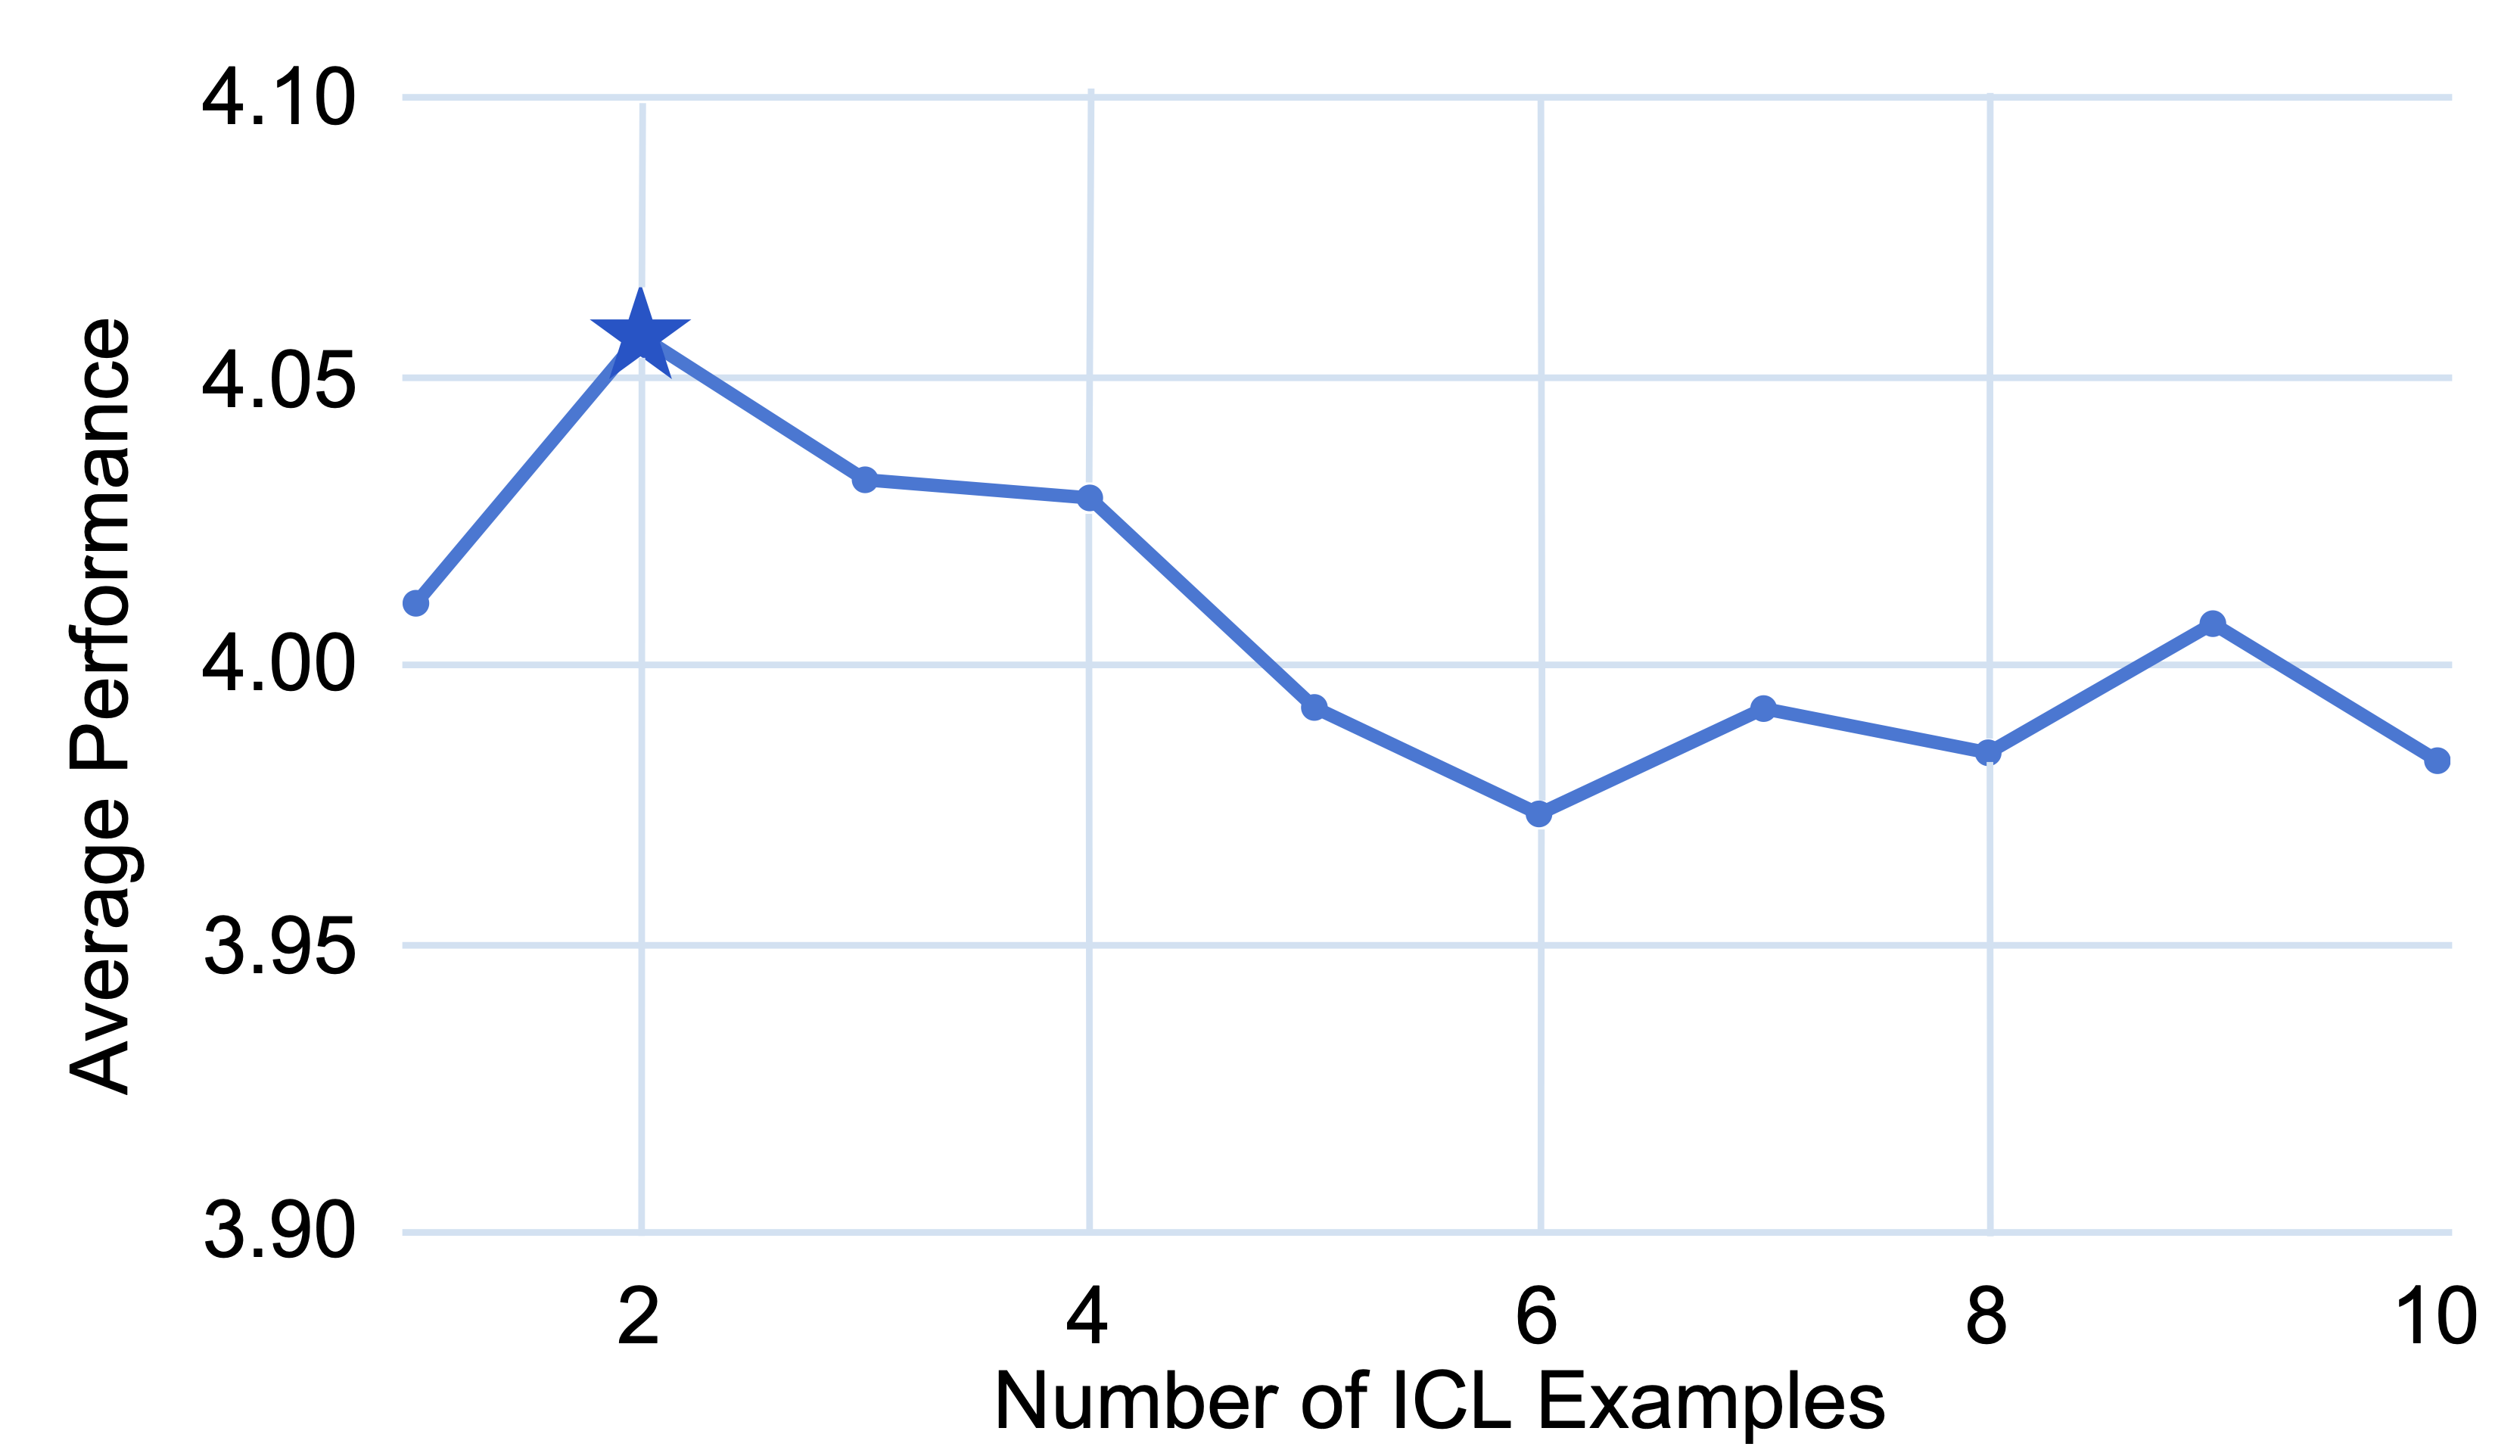
\includegraphics[ width=\linewidth]{images/icl_variation_line_chart_white_bg_v2.png}
    \caption{Performance of Mistral 7b (Instruct)  on varying the number of ICL examples. Two examples give us the best performance with a lower context length cost.}
    \label{fig:icl_variation_chart}
    \vspace{-5pt}
\end{figure}



% Qualitative analysis of gpt prompt

\newcommand{\reduline}[1]{{\color{red}\underline{{\color{black}#1}}}}

\newcommand\dunderline[2][.2pt]{\raisebox{-#1}{\underline{\raisebox{#1}{\smash{\underline{#2}}}}}}

\begin{table}[!t]

\definecolor{Gray}{gray}{0.90}
\newcolumntype{a}{>{\columncolor{Gray}}c}
\centering
\resizebox{1\linewidth}{!}{%
\begin{tabular}{@{}p{10cm}@{}}
\toprule
\textbf{Optimized Alignment Prompt} \\
\midrule
As a helpful and ethical assistant, your primary goal is to provide responses that are accurate, engaging, clear, and emotionally resonant across a wide range of queries. \\
- \ctext[RGB]{230,246,255}{Strive to make complex topics understandable and emotionally engaging, communicating in a human-like and relatable manner. Organize your responses to enhance readability and emotional connection, avoiding overly technical jargon.}  \\
- \ctext[RGB]{233,252,232}{Always acknowledge the limitations of your knowledge, especially when speculating about historical 'what-ifs', future predictions, or interpreting emotions.} \\
- \ctext[RGB]{255,225,255}{Aim for a balance between detailed, informative content and a conversational, engaging tone. Incorporate storytelling elements, examples, analogies, and direct questions to make information relatable.} \\
- \ctext[RGB]{230,246,255}{Avoid overwhelming the user with excessive information; structure your responses to be clear, well-organized, and mindful of the user's cognitive load.}
 \\

 \bottomrule
\end{tabular}%
}
 
\caption{Snippets from the system prompt optimized for \texttt{gpt-3.5-turbo}. The optimized prompt clearly demonstrates improved alignment, addressing potential weaknesses in the model.}
\label{tab:gpt_prompt}
\vspace{-15pt}
\end{table}
\noindent \textbf{Qualitative analysis of optimized prompts}. 
We finally present qualitative results to show \ours' ability to identify a model's alignment weaknesses and tailor system prompts to address them, as shown in Table \ref{tab:gpt_prompt} for \texttt{gpt-3.5-turbo}. The color-coded text in the table highlights specific weaknesses of \texttt{gpt-3.5-turbo} identified by \ours, along with actionable insights. Notably, it highlights \ctext[RGB]{233,252,232}{knowledge limitations of the model}, \ctext[RGB]{255,225,255}{tips to improve engagement} and \ctext[RGB]{230,246,255}{technical verbiage}. For a weaker model like Mistral 7b, \ours identifies the problem of repetitive tokens, which is absent in a strong model like \texttt{gpt-3.5-turbo}. Complete optimized prompts for both models, along with detailed annotations on the differences, can be found in Appendix \ref{sec:prompt_case_study}.  

% radar chart, analyzing various domains/dimensions 
